\section{Estabilidad y deformaci\'{o}n de un d\'{u}plex de ADN: predicci\'{o}n de promotores} \label{dna1}
 
 
El modelo \italics{Nearest Neighbor} (NN) aproxima la estabilidad termodin\'{a}mica de un \'{a}cido nucleico en disoluci\'{o}n
a partir de su secuencia, que se analiza como una secuencia de dinucle\'{o}tidos solapantes 
de interacciones aditivas, cuyas energ\'{i}as se han determinado experimentalmente \citep{Breslauer1986,SantaLucia1998}.

\begin{figure}
\begin{center} 
\includegraphics{NN}
\caption{C\'{a}lculo de estabilidad (energ\'{i}a libre de Gibbs, $\Delta G$) a temperatura fisiol\'{o}gica en base al modelo NN, 
incluyendo un t\'{e}rmino de iniciaci\'{o}n de d\'{u}plex, tomado de \citep{SantaLucia1998}.
Copyright (1998) National Academy of Sciences.
}
\label{fig:NN}
\end{center}
\end{figure}

Inspir\'{a}ndose en estructuras moleculares conocidas, 
este tipo de modelos se han empleado para describir la lectura indirecta del DNA, por su forma, 
por parte de nucleosomas \citep{Heijden2012} o factores de transcripci\'{o}n \citep{Gromiha2004,Espinosa2008}.

\begin{figure}
\begin{center} 
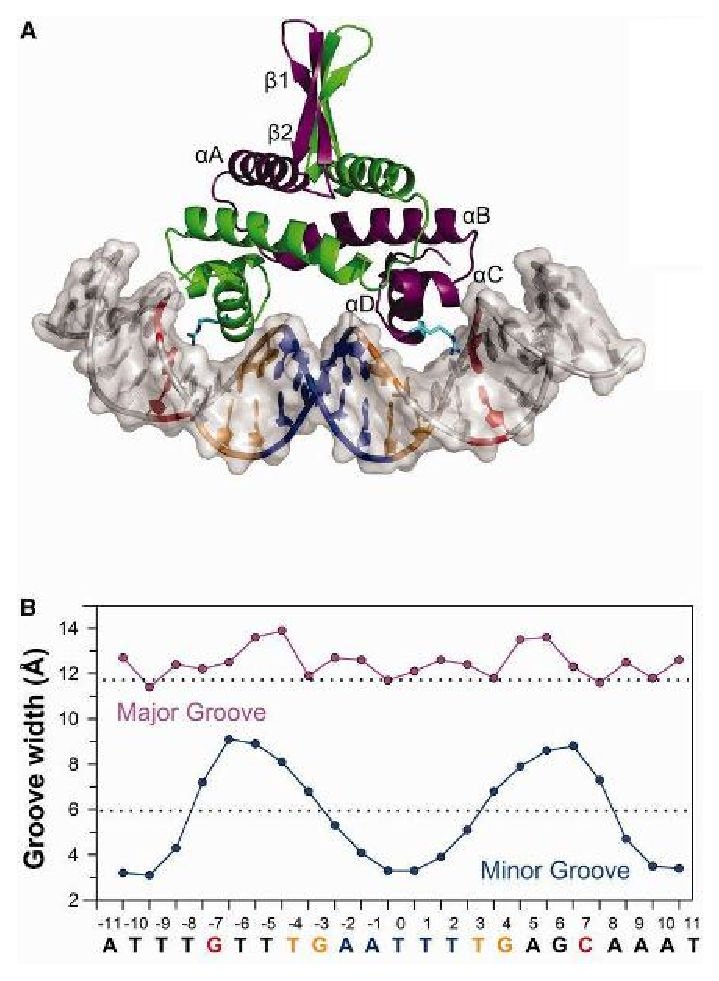
\includegraphics{MGW}
\caption{
(A) Estructura de un homod\'{i}mero de Fis unido a un sitio de alta afinidad 
(PDB: \htmladdnormallink{3IV5}{http://www.rcsb.org/structure/3IV5}), 
insertando dos h\'{e}lices en dos surcos mayores consecutivos. 
(B) Ancho del surco mayor (magenta) y menor (MGW, azul) a lo largo de la secuencia de DNA medido entre los fosfatos m\'{a}s cercanos.
Las lineas punteadas representan los valores can\'{o}nicos para B-DNA. 
Figura adaptada de \citet{Hancock2013} y reproducida con permiso de los autores.}
\label{fig:MGW}
\end{center}
\end{figure}

\begin{figure}
\begin{center} 
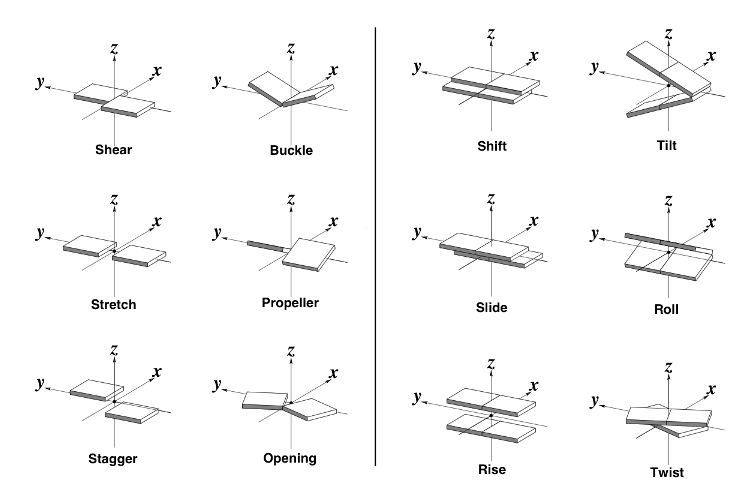
\includegraphics{BPgeom}
\caption{
Propiedades de pares de bases (izquierda) y dinucle\'{o}tidos (derecha) que se pueden estimar a partir de la estructura. 
Figura tomada de \htmladdnormallink{x3dna.org}{http://x3dna.org/articles/seeing-is-understanding-as-well-as-believing}.}
\label{fig:BPgeometry}
\end{center}
\end{figure}

%\begin{figure}
%\begin{center} 
%\includegraphics{DNAshape13}
%\caption{Propiedades de pares de bases y dinucle\'{o}tidos que se pueden estimar a partir de la estructura \citep{Li2017}.}
%\label{fig:DNAshape13}
%\end{center}
%\end{figure}



Otros modelos ampl\'{i}an el n\'{u}mero de vecinos considerados hasta llegar, por ejemplo, a pent\'{a}meros:

\begin{figure}
\begin{center} 
\includegraphics{DNApentamers}
\caption{Aproximaci\'{o}n de propiedades estructurales (MGW=minor groove width) de un d\'{u}plex de ADN por solapamiento de pent\'{a}meros, 
base del algoritmo \htmladdnormallink{DNAshape}{http://rohsdb.cmb.usc.edu}. 
Reproducido con permiso de \citet{Zhou2013}.
Este tipo de aproximaciones se est\'{a}n usando para enriquecer motivos de DNA reconocidos por factores de transcripci\'{o}n \citep{Yang2015}}
\label{fig:NN5}
\end{center}
\end{figure}

En esta secci\'{o}n aplicaremos el modelo NN a la predicci\'{o}n de promotores:

\begin{itemize}
\item \textbf{PROBLEMA:} disponemos de coordenadas gen\'{o}micas de una colecci\'{o}n de marcos de lectura 
(\htmladdnormallink{\italics{Open Reading Frames, ORFs}}{http://es.wikipedia.org/wiki/Marco_abierto_de_lectura}), 
pero desconocemos la posici\'{o}n de sus secuencias promotoras
\item \textbf{SOLUCI\'{O}N PROPUESTA:} buscar los promotores en la secuencia del DNA por su menor estabilidad termodin\'{a}mica
\end{itemize}

Este problema ha tenido mayor importancia en procariotas por la gran velocidad con que se han ido obteniendo sus secuencias gen\'{o}micas, 
y el algoritmo de \cite{Kanhere2005} es un ejemplo de como emplear una estrategia estructural para atacar este problema. 
El algoritmo consiste en estimar la estabilidad helicoidal del ADN cromos\'{o}mico, que se supone es menor en
las regiones promotoras, donde la maquinaria transcripcional se asienta para comenzar la s\'{i}ntesis de ARN. 
En concreto este m\'{e}todo estima la estabilidad de una (ventana de) secuencia de ADN a ambos lados de una coordenada y define como posibles
posiciones promotores aquellas donde la diferencia de estabilidad en torno a una coordenada es significativa. 

\begin{figure}
\begin{center} 
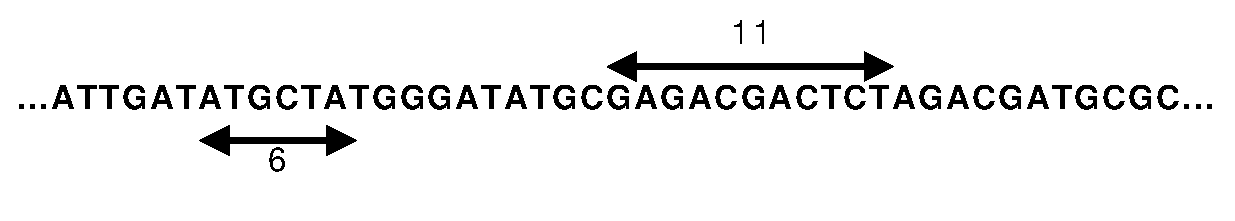
\includegraphics{window}
\caption{Ejemplos de ventanas de 6 y 11 nucle\'{o}tidos, que sirven para promediar propiedades a lo largo de la secuencia.}
\label{fig:window}
\end{center}
\end{figure}

Este algoritmo incluye varios par\'{a}metros libres y en el art\'{i}culo original se muestra como entrenarlo para obtener valores adecuados para todos ellos.

\begin{figure}
\begin{center} 
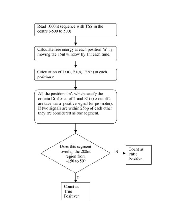
\includegraphics{flowKanhere}
\caption{Algoritmo de \cite{Kanhere2005}, que se basa en calcular la diferencia de $\Delta G$ entre dos ventanas en torno a una posici\'{o}n $n$.
Figura reproducida con permiso de los autores.}
\label{fig:Kanhere}
\end{center}
\end{figure}

Se han propuesto otras aproximaciones estructurales, como la de \cite{Gogni2007}, %(\htmladdnormallink{PDF}{./papers/euk_promoter_prediction2007.pdf})
que identifica regiones promotoras en base a la capacidad de deformaci\'{o}n de los 
\htmladdnormallink{pares de bases}{http://nar.oxfordjournals.org/content/31/17/5108/F1.large.jpg},
estimada por medio de extensas simulaciones moleculares precalculadas. 
%Sin duda \'{e}sta es un \'{a}rea de investigaci\'{o}n en crecimiento y constantemente se siguen publicando 
%\htmladdnormallink{nuevos trabajos}{http://www.ncbi.nlm.nih.gov/pubmed?term=structural[All Fields] AND prediction[All Fields] AND promoters[All Fields]}. 

El repertorio de m\'{e}todos para predicci\'{o}n de promotores en base a inferencias estructurales es limitado, pero incluye al menos: 
\htmladdnormallink{proStar}{http://mmb.pcb.ub.es/proStar/}, \htmladdnormallink{ProSOM}{http://bioinformatics.psb.ugent.be/software/details/ProSOM}
%\htmladdnormallink{profisi}{http://mlg.ucd.ie/profisi} 
o el algoritmo de \citet{Song2012}. Otras opciones recientes se basan en combinar diferentes fuentes por medio de algoritmos de aprendizaje \citep{Eser2016}.

El ejercicio de esta secci\'{o}n consiste en completar el siguiente programa, usando los par\'{a}metros unificados de \cite{SantaLucia1998},
para calcular la diferencia de estabilidad $D(n)$ entre dos fragmentos de 50bp y 100bp $E1(n)$ y $E2(n)$ 
que flanquean una regi\'{o}n central (de 50bp) que podr\'{i}a albergar el promotor.
A su vez, estos framentos se calculan sobre valores de estabilidad calculados sobre ventanas de secuencia 
de longitud 15pb en el art\'{i}culo de \cite{Kanhere2005}:

\begin{equation}
E1(n) = \frac{\sum_{n}^{n+49}\Delta G}{50} 
\end{equation}

\begin{equation}
E2(n) = \frac{\sum_{n+99}^{n+199}\Delta G}{100} 
\end{equation}

\begin{equation}
D(n) = E1(n) - E2(n)
\end{equation}

Como conjunto de datos para la predicci\'{o}n de promotores usaremos las secuencias del fichero \htmladdnormallink{K12\_400\_50\_sites}{./files/K12_400_50_sites}, 
que contiene coordenadas de ORFs de \italics{Escherichia coli} con coordenadas -400,+50, con el 0 centrado cerca del cod\'{o}n de inicio.
Qu\'{e} observas al cambiar el tama\~no de la ventana?
\verbatiminput{code/prog1.1.pl}
